% !TEX root = ../main.tex
\chapter{Numerical Implementation}
\label{app:numerical_implementation}

This appendix records the numerical conventions and implementation details used
to obtain the results of this thesis. The calculations employ \texttt{QuTiP}
for the open-system time evolution~\cite{lambertetal2026qutip5quantum}. In
agreement with~\cref{chapter:spctr_spectroscopy,chapter:oqs_open_quantum_systems,chapter:model_systems},
it summarises the pulse and bath conventions, operator construction, signal
assembly, and post-processing steps used throughout this work.

\section{Overview}
\label{app:sec:software_architecture}

Each simulation run proceeds through four stages:
\begin{enumerate}
    \item the chosen physical parameters are converted into a concrete
    Hamiltonian, pulse sequence, bath model, and numerical setup;
    \item for each chosen coherence time and each inhomogeneous realisation,
    the density matrix is propagated under the complete three-pulse sequence;
    \item the emitted third-order field is obtained by one-pulse subtraction
    and discrete phase cycling;
    \item the time-domain signals are averaged over disorder and Fourier
    transformed into the final 1D or 2D spectra.
\end{enumerate}

The workflow therefore keeps the physical model explicit throughout; the
remaining numerical steps only evaluate it.

\section{Units and Time Axes}
\label{app:sec:configuration_workflow}

\subsection{Internal Units}

Transition frequencies are specified in \si{\per\centi\metre}, but the dynamics
are propagated in angular-frequency units of \si{\per\femto\second}. Internally,
the conversion is
\[
\omega_{\mathrm{fs}^{-1}}
=
2\pi c \cdot 10^{-5}\,\omega_{\mathrm{cm}^{-1}}.
\]
The same convention is used for site energies, couplings, pulse carrier
frequencies, and bath frequencies. In the code, \(\hbar\) is set to unity, so
Hamiltonian matrix elements are numerically expressed in the same
\(\mathrm{fs}^{-1}\) units.

The bath sector is parameterised through the dimensionless ratios
\(T/\bar{\omega}_0\), \(\omega_{\mathrm{c}}/\bar{\omega}_0\), and
\(\alpha/\bar{\omega}_0\), where
\[
\bar{\omega}_0
=
\frac{1}{N_{\mathrm{sites}}}
\sum_{i=1}^{N_{\mathrm{sites}}}\omega_i
\]
is a characteristic optical scale. The code reconstructs the corresponding
dimensional quantities before constructing the QuTiP environment, for example
through
\[
T
=
\left(\frac{T}{\bar{\omega}_0}\right)\bar{\omega}_0,
\qquad
\omega_{\mathrm{c}}
=
\left(\frac{\omega_{\mathrm{c}}}{\bar{\omega}_0}\right)\bar{\omega}_0.
\]

\subsection{Time Grids and Pulse Timing}

The public coherence and detection axes begin at zero. The solver-local time
grid starts earlier so that the first pulse is already present when the
propagation begins.

The delays \(t_{\mathrm{coh}}\), \(t_{\mathrm{wait}}\), and
\(t_{\mathrm{det}}\) follow the collinear three-pulse convention introduced
in~\autoref{fig:spctr_fwm_phase_cycling_setup} and discussed
in~\autoref{sec:spctr_phase_cycling}. For given \(t_{\mathrm{coh}}\) and
\(t_{\mathrm{wait}}\), the pulse peaks are placed at
\[
t_1 = -(t_{\mathrm{coh}} + t_{\mathrm{wait}}),
\qquad
t_2 = -t_{\mathrm{wait}},
\qquad
t_3 = 0.
\]

The solver-local initial time is chosen to lie before the first pulse window.
In principle this could be \(-\infty\), because the system starts in a thermal
state. For Gaussian pulses, however, the code uses
\[
t_0
=
-\Bigl(t_{\mathrm{coh}} + t_{\mathrm{wait}} + 1.823\,\tau_{\mathrm{p}}\Bigr),
\]
rounded down to the nearest multiple of the stored output spacing
\texttt{dt}. The factor \(1.823\) is the active half-width used in the laser
module; at this cutoff the Gaussian intensity has already dropped below
\(10^{-4}\) of its peak value.

The stored output spacing is set by \texttt{dt}. The adaptive solver step size
is controlled separately through \texttt{max\_step}. Internally,
\texttt{max\_step} is chosen so that the pulse envelope is resolved
sufficiently in RWA runs and the optical carrier is resolved sufficiently in
full laboratory-frame runs. Because the pulses have finite duration, this
timing convention also produces a short-waiting-time pulse-overlap regime. Its
spectroscopic consequences are discussed
in~\autoref{subsec:results_monomer_2d_freq}
and~\autoref{subsec:results_dimer_waiting_time}.

\section{Operator Representations}
\label{app:sec:model_systems}

\subsection{Basis Indexing}

The basis states defined in~\autoref{sec:model_ensemble} are stored on an
explicit ordered index set. For a model with \(N_{\mathrm{sites}}\) sites, the
ordered basis begins with the ground state, continues with the
\(N_{\mathrm{sites}}\) single-excitation states, and, when retained, appends
the double-excitation states \(\ket{ij}\) with \(i<j\). Thus the numerical
basis has the same three-band structure as in the model chapter:
\(\ket{\mathrm{g}}\), \(\{\ket{i}\}\), and \(\{\ket{ij}\}\). Because each site is a
two-level system, \(\ket{ij}\) always denotes excitations on two different
sites. The pair states are ordered deterministically, so the mapping from a
site pair \((i,j)\) to the basis index of \(\ket{ij}\) is fixed across runs.
This convention ensures that the same stored parameter set reconstructs the
same Hamiltonian and dipole matrices reproducibly.

\subsection{Eigenbasis Transformation}

The energy eigenbasis is obtained by diagonalising the Hamiltonian. If \(U\)
denotes the resulting unitary transformation, operators are first constructed
in the site basis and then transformed as
\[
\hat{O}_{\mathrm{eig}} = U^{\dagger}\hat{O}_{\mathrm{site}}U.
\]
The field-free Hamiltonian, the dipole operator, and the coupling operators
from~\autoref{sec:model_ensemble} are stored in this basis. The eigenvectors
are additionally phase-fixed numerically so that the first nonzero component of
each eigenvector is real and positive. This makes stored eigenbasis quantities
reproducible across runs.

\section{Laser Pulses and Light-Matter Interaction}
\label{app:sec:laser_field}

The pulse model stores three pulses with amplitudes \(A_k\), phases \(\phi_k\),
common carrier frequency \(\omega_{\mathrm{L}}\), a chosen envelope type, and FWHM
\(\tau_{\mathrm{p}}\). The implemented three-pulse field convention follows the
main-text definitions of the applied field and its positive- and
negative-frequency decomposition
in~\cref{eq:spctr_E_three_pulses_space,eq:spctr_E_plusminus}. The only
additional numerical ingredient is the truncation of the envelope to finite
support.

Two envelope types are implemented: Gaussian and \(\cos^2\). For Gaussian
pulses, the envelope
\begin{equation}
\label{eq:laser_envelope}
s_k(t)
=
\exp\!\left[
-\frac{(t-t_k)^2}{2\sigma^2}
\right],
\qquad
\sigma
=
\frac{\tau_{\mathrm{p}}}{2\sqrt{2\ln 2}},
\end{equation}
is evaluated only inside the active window
\([t_k-1.823\tau_{\mathrm{p}},\,t_k+1.823\tau_{\mathrm{p}}]\). Inside this
window, the boundary value is subtracted,
\[
s_k^{\mathrm{num}}(t)
=
\max\!\bigl(s_k(t)-s_k(t_k \pm 1.823\tau_{\mathrm{p}}),0\bigr),
\]
so that the truncated envelope vanishes continuously at the numerical cutoff.
Outside the active window, the field is set to zero.

The implementation distinguishes between the full laboratory-frame
positive-frequency field and its slowly varying envelope. The scalar dipole
Hamiltonian of~\autoref{eq:spctr_semiclassical_hamiltonian_scalar} is therefore
implemented either with the full laboratory-frame field or, in RWA runs, with
the decomposition of~\autoref{eq:spctr_E_plusminus}. In the internal notation,
\[
\varepsilon^{(+)}(t)
=
e^{-i\omega_{\mathrm{L}} t} E(t),
\qquad
E(t)
=
\sum_{k=1}^{3} A_k s_k(t)e^{-i\phi_k},
\]
where \(\omega_{\mathrm{L}}\) is the common carrier frequency and \(\phi_k\) are the
phase-cycling phases. The non-RWA implementation uses the full field
\(\varepsilon^{(+)}(t)\) and the full dipole operator,
\[
H_{\mathrm{int}}(t)
=
-\hat{\mu}\Bigl(\varepsilon^{(+)}(t)+\varepsilon^{(-)}(t)\Bigr),
\]
whereas the RWA implementation uses the slowly varying envelope,
\begin{equation}
\label{eq:app_rwa_interaction_hamiltonian}
H_{\mathrm{int}}^{\mathrm{RWA}}(t)
=
-\Bigl(\hat{\mu}^{(-)}E^{*}(t)+\hat{\mu}^{(+)}E(t)\Bigr).
\end{equation}
This is the convention used both by the generic Hamiltonian treatment and by
the explicit equations of motion.

\section{Open Quantum System Terms}
\label{app:sec:oqs_evolution}

\subsection{Initial State}

The default initial state is the ground-state density matrix. For
finite-temperature Redfield calculations, the code can also construct a
Boltzmann state in the energy eigenbasis,
\[
\rho_{\mathrm{th}}
=
\frac{1}{Z}\sum_{a} e^{-E_a/T}\ket{a}\!\bra{a},
\]
but this option is restricted to Redfield runs, because only that backend
treats finite-temperature equilibration consistently. This construction
specialises the Gibbs-state form of~\autoref{eq:oqs_ho_gibbs_state} to the
system eigenbasis used by the solver.

\subsection{Explicit Equations of Motion}
\label{app:sec:paper_eqs_explicit_eoms}

For direct comparison with the monomer and dimer benchmark literature, the
workflow also provides a hard-coded implementation of the corresponding
equations-of-motion form used
in~\cite{mancaletal2006twodimensionalopticalthreepulse,pisliakovetal2006twodimensionalopticalthreepulse}.

\noindent\textbf{Monomer equations.}

Using the rotating-frame ansatz
\[
\rho_{\mathrm{eg}}(t)=\sigma_{\mathrm{eg}}(t)\,\mathrm{e}^{-\mathrm{i}\omega_{\mathrm{L}} t},
\qquad
\rho_{\mathrm{ge}}(t)=\sigma_{\mathrm{ge}}(t)\,\mathrm{e}^{+\mathrm{i}\omega_{\mathrm{L}} t},
\]
the implemented monomer equations are
\begin{align}
\dot{\sigma}_{\mathrm{eg}}
&=
-\bigl(\Gamma + i\Delta_{\mathrm{L}}\bigr)\sigma_{\mathrm{eg}}
+ i\,\mu_{\mathrm{eg}} E(t)\,\bigl(\rho_{\mathrm{gg}}-\rho_{\mathrm{ee}}\bigr),
\label{eq:app_monomer_eom_sigma_eg}
\\
\dot{\rho}_{\mathrm{ee}}
&=
-\gamma_{\downarrow}\rho_{\mathrm{ee}}
+ \gamma_{\uparrow}\rho_{\mathrm{gg}}
+ i\,\mu_{\mathrm{eg}}E(t)\sigma_{\mathrm{ge}}
- i\,\mu_{\mathrm{eg}}E^{*}(t)\sigma_{\mathrm{eg}},
\notag
\\
\dot{\rho}_{\mathrm{gg}}
&=
-\gamma_{\uparrow}\rho_{\mathrm{gg}}
+ \gamma_{\downarrow}\rho_{\mathrm{ee}}
- i\,\mu_{\mathrm{eg}}E(t)\sigma_{\mathrm{ge}}
+ i\,\mu_{\mathrm{eg}}E^{*}(t)\sigma_{\mathrm{eg}}.
\label{eq:app_monomer_eom_rho_gg}
\end{align}
Here,
\[
\Gamma
=
\gamma_{\varphi}+\frac{\gamma_{\downarrow}+\gamma_{\uparrow}}{2},
\qquad
\Delta_{\mathrm{L}}
=
\omega_{\mathrm{eg}}-\omega_{\mathrm{L}}.
\]
For the monomer runs used here, \(\gamma_{\uparrow}=0\), so the equations
reduce to the familiar phenomenological monomer form used in the main results
chapter.

\noindent\textbf{Dimer equations.}

For the dimer backend, the relevant exciton-basis dipole matrix elements are
\(\mu_{10}\), \(\mu_{20}\), \(\mu_{31}\), and \(\mu_{32}\). These are the
adjacent-manifold couplings introduced in~\autoref{sec:model_dimer} and
summarised in~\autoref{fig:rslts_dimer_basis_map}. The transition frequencies
are \(\omega_{ab}=E_a-E_b\). The damping and transfer rates are not inserted
phenomenologically, but are deduced from the Redfield tensor of the microscopic
bath model introduced in
~\cref{eq:oqs_Interaction_Hamiltonian,eq:oqs_Rabcd_full} and evaluated through
the bath power spectrum~\cref{eq:oqs_Noise_Power_Spectrum}.

The rotating-frame ansatz is
\[
\rho_{10}=\sigma_{10}\mathrm{e}^{-\mathrm{i}\omega_{\mathrm{L}} t},
\quad
\rho_{20}=\sigma_{20}\mathrm{e}^{-\mathrm{i}\omega_{\mathrm{L}} t},
\quad
\rho_{30}=\sigma_{30}\mathrm{e}^{-2\mathrm{i}\omega_{\mathrm{L}} t},
\quad
\rho_{31}=\sigma_{31}\mathrm{e}^{-\mathrm{i}\omega_{\mathrm{L}} t},
\quad
\rho_{32}=\sigma_{32}\mathrm{e}^{-\mathrm{i}\omega_{\mathrm{L}} t},
\]
while the intraband coherence \(\rho_{12}\) and the populations \(\rho_{aa}\)
are left unchanged. In this notation the implemented equations read
\begin{align*}
\dot{\sigma}_{10}
&=
-\bigl[i(\omega_{10}-\omega_{\mathrm{L}})+\Gamma_{10}\bigr]\sigma_{10}
+ iE(t)\bigl[\mu_{10}(\rho_{00}-\rho_{11})-\mu_{20}\rho_{12}\bigr]
+ iE^{*}(t)\mu_{31}\sigma_{30},
\\
\dot{\sigma}_{20}
&=
-\bigl[i(\omega_{20}-\omega_{\mathrm{L}})+\Gamma_{20}\bigr]\sigma_{20}
+ iE(t)\bigl[\mu_{20}(\rho_{00}-\rho_{22})-\mu_{10}\rho_{21}\bigr]
+ iE^{*}(t)\mu_{32}\sigma_{30},
\\
\dot{\sigma}_{30}
&=
-\bigl[i(\omega_{30}-2\omega_{\mathrm{L}})+\Gamma_{30}\bigr]\sigma_{30}
+ iE(t)\bigl[\mu_{31}\sigma_{10}+\mu_{32}\sigma_{20}
- \mu_{10}\sigma_{31}-\mu_{20}\sigma_{32}\bigr],
\\
\dot{\sigma}_{31}
&=
-\bigl[i(\omega_{31}-\omega_{\mathrm{L}})+\Gamma_{31}\bigr]\sigma_{31}
+ iE(t)\bigl[\mu_{31}(\rho_{11}-\rho_{33})+\mu_{32}\rho_{21}\bigr]
- iE^{*}(t)\mu_{10}\sigma_{30},
\\
\dot{\sigma}_{32}
&=
-\bigl[i(\omega_{32}-\omega_{\mathrm{L}})+\Gamma_{32}\bigr]\sigma_{32}
+ iE(t)\bigl[\mu_{32}(\rho_{22}-\rho_{33})+\mu_{31}\rho_{12}\bigr]
- iE^{*}(t)\mu_{20}\sigma_{30},
\\
\dot{\rho}_{12}
&=
-\bigl(i\omega_{12}+\Gamma_{12}\bigr)\rho_{12}
+ iE(t)\bigl[\mu_{10}\sigma_{02}-\mu_{32}\sigma_{13}\bigr]
+ iE^{*}(t)\bigl[\mu_{31}\sigma_{32}-\mu_{20}\sigma_{10}\bigr],
\\
\dot{\rho}_{11}
&=
-\Gamma_{11}\rho_{11}
+ \gamma_{12}\rho_{22}
+ iE(t)\bigl[\mu_{10}\sigma_{01}-\mu_{31}\sigma_{13}\bigr]
+ iE^{*}(t)\bigl[\mu_{31}\sigma_{31}-\mu_{10}\sigma_{10}\bigr],
\\
\dot{\rho}_{22}
&=
-\Gamma_{22}\rho_{22}
+ \gamma_{21}\rho_{11}
+ iE(t)\bigl[\mu_{20}\sigma_{02}-\mu_{32}\sigma_{23}\bigr]
+ iE^{*}(t)\bigl[\mu_{32}\sigma_{32}-\mu_{20}\sigma_{20}\bigr],
\\
\dot{\rho}_{00}
&=
-iE(t)\bigl[\mu_{10}\sigma_{01}+\mu_{20}\sigma_{02}\bigr]
+ iE^{*}(t)\bigl[\mu_{10}\sigma_{10}+\mu_{20}\sigma_{20}\bigr].
\end{align*}

The rates entering these equations can be written in terms of the dimer mixing
angle \(\theta\) from~\autoref{eq:dimer_mixing_angle} and the bath power
spectrum \(\mathcal{S}(\omega)\) as
\begin{align*}
\gamma_{12} &= \sin^{2}(2\theta)\,\mathcal{S}(\omega_{21}),
\qquad
\gamma_{21} = \sin^{2}(2\theta)\,\mathcal{S}(\omega_{12}),
\\
\Gamma_{10} &= \Gamma_{31}
= \left(1-\frac{1}{2}\sin^{2}(2\theta)\right)\mathcal{S}(0)
+ \frac{\gamma_{21}}{2},
\\
\Gamma_{20} &= \Gamma_{32}
= \left(1-\frac{1}{2}\sin^{2}(2\theta)\right)\mathcal{S}(0)
+ \frac{\gamma_{12}}{2},
\\
\Gamma_{30} &= 2\mathcal{S}(0),
\qquad
\Gamma_{12} = 2\cos^{2}(2\theta)\,\mathcal{S}(0)
+ \frac{\gamma_{12}+\gamma_{21}}{2},
\\
\Gamma_{11} &= \gamma_{21},
\qquad
\Gamma_{22} = \gamma_{12}.
\end{align*}
This is the Appendix-C form used for the hard-coded dimer benchmark equations
in Paper~II, but here written explicitly in terms of the underlying Redfield
rates instead of leaving the \(\Gamma_{ij}\) implicit.

The remaining relations are fixed by Hermiticity and normalisation:
\[
\rho_{21}=\rho_{12}^{*},
\qquad
\sigma_{01}=\sigma_{10}^{*},
\qquad
\sigma_{02}=\sigma_{20}^{*},
\qquad
\sigma_{13}=\sigma_{31}^{*},
\qquad
\sigma_{23}=\sigma_{32}^{*},
\qquad
\dot{\rho}_{33}
=
-\dot{\rho}_{00}-\dot{\rho}_{11}-\dot{\rho}_{22}.
\]

This explicit \(16\times16\) construction makes one implementation detail more
transparent than the shortened printed list in Paper~II. There, only the subset
(D1)--(D6) is written explicitly, and the remaining one-exciton equations are
generated by the substitution \(1\leftrightarrow2\). In the full RWA
commutator, however, the coherences \(\sigma_{31}\) and \(\sigma_{32}\) also
contain terms proportional to the upper-manifold population \(\rho_{33}\). The
implemented equations therefore retain the completed commutator form rather
than a literal transcription of the shortened printed appendix:
\[
iE(t)\bigl[\mu_{31}(\rho_{11}-\rho_{33})+\mu_{32}\rho_{21}\bigr],
\qquad
iE(t)\bigl[\mu_{32}(\rho_{22}-\rho_{33})+\mu_{31}\rho_{12}\bigr].
\]

\subsection{Solver Diagnostics and Time Cutoff}

Because Redfield dynamics can produce unphysical density matrices, the workflow
first performs a diagnostic run before the full simulation. It uses the maximal
configured coherence time \(t_{\mathrm{coh,max}}\), fixes the pulse phases to
\((\phi_1,\phi_2,\phi_3)=(0,0,0)\), propagates one trajectory, and checks at
every stored time point whether the density matrix remains Hermitian, trace
preserving, and positive semidefinite.

The positivity test is implemented with a numerical tolerance,
\[
\lambda_{\min}(\rho(t)) \ge -10^{-6},
\]
where \(\lambda_{\min}\) denotes the smallest eigenvalue of the propagated
density matrix. The first time at which Hermiticity, positivity, or trace
preservation fails defines a numerical cutoff time \(t_{\mathrm{cut}}\). The
emitted field is then multiplied by a mask that sets the signal to zero for
\(t_{\mathrm{det}} > t_{\mathrm{cut}}\). This does not guarantee that every
possible trajectory remains physical, but it provides an important safeguard.

Once a configuration has passed at \(t_{\mathrm{coh,max}}\), the resulting
\(t_{\mathrm{cut}}\) is stored and reused during the full signal construction.
For all generated results, the diagnostic remained successful, so that
\(t_{\mathrm{cut}}=\infty\).

The same trajectory-level analysis is also useful for quantifying how much
secularisation changes an otherwise fixed Redfield simulation
(see~\autoref{subsec:oqs_Fourier_and_secular}).

For two arbitrary density operators \(\rho\) and \(\sigma\), the trace distance
is defined as
\[
D_{\mathrm{tr}}(\rho,\sigma)
=
\frac{1}{2}\left\|\rho-\sigma\right\|_1,
\]
with trace norm
\[
\|A\|_1
=
\mathrm{Tr}\!\left[\sqrt{A^{\dagger}A}\right].
\]

In~\autoref{fig:app_dimer_redfield_sec_cutoff_diagnostic}, the physical
parameters match the coupled dimer discussed
in~\autoref{subsec:results_dimer_coupled_case}; only the dissipative treatment
is switched between full Bloch--Redfield and secular Bloch--Redfield. The
stored output spacing is \(\Delta t=\SI{1}{\femto\second}\), so that the driven
evolution is resolved clearly. Denoting the two trajectories by
\(\rho_{\mathrm{full}}(t)\) and \(\rho_{\mathrm{sec}}(t)\), the pointwise
comparison is
\(D_{\mathrm{tr}}(\rho_{\mathrm{full}}(t),\rho_{\mathrm{sec}}(t))\). To
summarise the full trajectory in two numbers, define
\[
D_{\max}
=
\max_t D_{\mathrm{tr}}(\rho_{\mathrm{full}}(t),\rho_{\mathrm{sec}}(t)),
\qquad
D_{\mathrm{mean}}
=
\frac{1}{t_f-t_i}\int_{t_i}^{t_f}
D_{\mathrm{tr}}(\rho_{\mathrm{full}}(t),\rho_{\mathrm{sec}}(t))\,dt.
\]

For the present pulse-driven coupled dimer trajectory, this gives
\(D_{\max}=3.03\times10^{-2}\) at \(t=\SI{17}{\femto\second}\) and
\(D_{\mathrm{mean}}=2.26\times10^{-2}\) over the stored solver-local
trajectory. The largest matrix-element change occurs in the ground-state
population \(\rho_{00}\), for which
\[
\max_t |\Delta\rho_{00}(t)| = 3.02\times10^{-2}.
\]
Thus, for this coupled dimer the secular approximation changes the driven
evolution at a clearly visible few-percent level, while the positivity
diagnostic remains safely above the numerical threshold and yields
\(t_{\mathrm{cut}}=\infty\).

\begin{figure}[htbp]
    \centering
    \safeplaceholdergraphic[0.98\linewidth]{figures/app_dimer_redfield_sec_cutoff_diagnostic}
    \caption{Diagnostic for secularisation in the coupled dimer. Top: time trace
    of the largest matrix-element difference between the full Bloch--Redfield
    and secular Bloch--Redfield trajectories. Middle: corresponding trace
    distance \(D_{\mathrm{tr}}\). Bottom: minimum eigenvalue of the propagated
    density matrix for the positivity diagnostic at
    \((\phi_1,\phi_2,\phi_3)=(0,0,0)\).}
    \label{fig:app_dimer_redfield_sec_cutoff_diagnostic}
\end{figure}

\section{Construction of the Third-Order Signal}
\label{app:sec:third_order_polarisation}

\subsection{Positive-Frequency Polarisation}

After propagation, the emitted signal is extracted from the density matrix
through the positive-frequency part of the dipole operator,
\[
P^{(+)}(t)
=
\mathrm{Tr}\!\left[\hat{\mu}^{(+)}\rho(t)\right].
\]
This is the implementation of the microscopic dipole expectation value
from~\autoref{eq:spctr_P_def_spectroscopy}, restricted to the radiating
positive-frequency component relevant for the emitted-field relation
in~\autoref{eq:spctr_signal_field_from_polarisation}.

In the implementation, \(\hat{\mu}^{(+)}\) is obtained by taking the strictly
lower-triangular part of the dipole matrix in the ordered eigenbasis. This
keeps only the radiating transitions between adjacent excitation sectors in the
ordering used by the code. The resulting signal is complex, so both amplitude
and phase are retained throughout the pipeline.

The solver-local trajectory is generally longer than the public detection
window. The code therefore computes the full propagated polarisation and then
slices it back onto the public detection axis
\(t_{\mathrm{det}} \in [0,T_{\mathrm{det}}]\). This keeps the pulse action and
the subsequent free evolution on one continuous internal grid while ensuring
that all saved artefacts use the same detection axis.

\subsection{One-Pulse Subtraction}

The implementation uses a non-perturbative three-pulse propagation, but the
desired observable is still the third-order response. To isolate it
numerically, the code evaluates, for every phase setting, one run with all
three pulses present and three auxiliary runs in which only a single pulse is
active. The background-subtracted signal is then
\begin{equation}
\label{eq:third_order_signal_numerical}
P^{(3)}(t)
\approx
P_{\mathrm{total}}(t)
- P_{(1)}(t)
- P_{(2)}(t)
- P_{(3)}(t).
\end{equation}
This is the implemented form of third-order isolation in the weak-field
regime. In the thesis calculations, the pulse amplitudes are chosen weak
enough that higher-order contamination remains numerically negligible. In weak
fields, this subtraction is the numerical counterpart of isolating the
third-order contribution \(P^{(3)}\)
in~\autoref{eq:spctr_P3_convolution_thesis} from the full driven response.

\subsection{Discrete Phase Cycling}

For a given coherence time and a given disorder realisation, the code evaluates
the phase grid
\[
\phi_1,\phi_2 \in
\left\{0,\frac{\pi}{2},\pi,\frac{3\pi}{2}\right\},
\qquad
\phi_3 = 0,
\]
which corresponds to the \(n_{\phi}=4\) phase-cycling grid used in the thesis
calculations. Here \(n_{\phi}\) denotes the number of sampled carrier phases
per pulse. The resulting discrete Fourier sum is the finite-grid realisation of
the carrier-phase projection derived
in~\autoref{eq:spctr_phase_cycling_projection} and used to isolate the
rephasing and nonrephasing classes discussed
in~\autoref{subsec:spctr_rephasing_nonrephasing}.

For each pair \((\phi_1,\phi_2)\), the one-pulse-subtracted signal is projected
onto the desired phase-matching component through
\[
P_{l,m}(t)
=
\left(\frac{\Delta\phi}{2\pi}\right)^2
\sum_{\phi_1,\phi_2}
e^{-i(l\phi_1 + m\phi_2)}
\Bigl[
P_{\mathrm{total}}(t;\phi_1,\phi_2)
- P_{(1)}(t;\phi_1)
- P_{(2)}(t;\phi_2)
- P_{(3)}(t)
\Bigr].
\]
The implementation uses \((l,m)=(-1,+1)\) for the rephasing contribution and
\((l,m)=(+1,-1)\) for the nonrephasing contribution. The emitted field is then
assembled as
\[
E_{\mathrm{sig}}(t) \propto -i\,P_{l,m}(t).
\]
This proportionality is the scalar implementation of the emitted-field relation
from~\autoref{eq:spctr_signal_field_from_polarisation}.

For fixed \((t_{\mathrm{coh}},n)\), one complete phase-cycling evaluation
therefore requires \(n_{\phi}^2 + 2n_{\phi} + 1\) separate propagations:
\(n_{\phi}^2\) full three-pulse runs, \(n_{\phi}\) single-pulse-1 runs,
\(n_{\phi}\) single-pulse-2 runs, and one single-pulse-3 run. These
propagations are mutually independent and can therefore be parallelised
directly.

\section{Ensembles with Inhomogeneous Broadening}
\label{app:sec:inhomogeneous_broadening}

The distinction between homogeneous and inhomogeneous broadening was introduced
in~\cref{sec:spctr_spectroscopy_motivation}. Static disorder is modelled
through Gaussian site-energy distributions with a common FWHM
\(\Delta_{\mathrm{inh}}\). For independent disorder, the implemented
single-site distribution is
\begin{equation}
\label{eq:gaussian_broadening}
p(\omega_i)
=
\frac{1}{\sigma\sqrt{2\pi}}
\exp\!\left[
-\frac{(\omega_i-\omega_{i,0})^2}{2\sigma^2}
\right],
\end{equation}
with
\[
\sigma
=
\frac{\Delta_{\mathrm{inh}}}{2\sqrt{2\ln 2}}.
\]

For realisation \(n\), the sampled site energy is written as
\[
\omega_i^{(n)}=\omega_{i,0}+\Delta_i^{(n)},
\]
where \(\Delta_i^{(n)}\) is the static detuning of site \(i\) in that
realisation. Independent sampling implies a factorised disorder distribution.
The cross-correlation therefore vanishes at the ensemble level,
\[
\langle \Delta_i \Delta_j\rangle_n = 0
\qquad
(i\neq j).
\]

Numerically, each site is sampled independently from its Gaussian
distribution. If \(\Delta_{\mathrm{inh}}=0\), the mean vector is used
directly. For each accepted realisation, the site-frequency vector is updated
before the Hamiltonian and the derived operators are rebuilt.

Each disorder realisation \(n\) is therefore a full sampled vector,
\[
\boldsymbol{\omega}^{(n)}
=
\bigl(\omega_1^{(n)},\omega_2^{(n)},\ldots,\omega_{N_{\mathrm{sites}}}^{(n)}\bigr).
\]
The propagation for realisation \(n\) uses only this vector. The sampling logic
is illustrated in~\autoref{fig:app_inhomogeneous_sampling_general}. For a
dimer, \(\omega_{\mathrm{A}}^{(n)}\) is therefore paired only with \(\omega_{\mathrm{B}}^{(n)}\),
not with \(\omega_{\mathrm{B}}^{(m)}\) for \(n\neq m\).

\begin{figure}[htbp]
    \centering
    \begin{tikzpicture}[x=1cm,y=1cm,>=latex]
        \tikzstyle{panel}=[draw=black!55, rounded corners=4pt, fill=black!2]

        \draw[panel] (-5.9,4.15) rectangle (5.9,5.75);
        \node[anchor=west,font=\small\bfseries] at (-5.6,5.47) {Independent site-resolved Gaussian sampling};

        \foreach \x/\lab in {-4.4/1,-1.5/2,1.4/3,4.3/{N_{\mathrm{sites}}}} {
            \draw[->,black!50] (\x-0.75,4.4) -- (\x+0.75,4.4);
            \draw[gray!60,densely dashed] (\x,4.4) -- (\x,5.18);
            \draw[thick,blue!70!black,samples=40,domain=-0.72:0.72,smooth,variable=\t]
                plot ({\x+\t}, {4.4 + 0.58*exp(-4.8*\t*\t)});
            \node[font=\scriptsize] at (\x,5.3) {$p_{\lab}(\omega_{\lab})$};
            \node[font=\scriptsize] at (\x,4.2) {$\omega_{\lab,0}$};
        }
        \node[font=\large] at (2.85,4.82) {$\cdots$};

        \draw[->,thick] (0,4.05) -- (0,3.55);

        \draw[panel] (-5.9,1.55) rectangle (5.9,3.55);
        \node[anchor=west,font=\small\bfseries] at (-5.6,3.25) {One accepted disorder realisation};

        \foreach \x/\y/\lab in {-4.4/2.88/1,-1.5/2.28/2,1.4/2.98/3,4.3/2.12/{N_{\mathrm{sites}}}} {
            \draw[gray!45] (\x,1.95) -- (\x,3.05);
            \fill[gray!70] (\x,2.52) circle (0.035);
            \fill[orange!85!black] (\x,\y) circle (0.06);
            \node[font=\scriptsize] at (\x,1.78) {site $\lab$};
        }
        \node[font=\large] at (2.85,1.78) {$\cdots$};
        \node[anchor=west,font=\scriptsize] at (4.7,3.0) {$\bullet$ sampled $\omega_i^{(n)}$};
        \node[anchor=west,font=\scriptsize,text=gray!70!black] at (4.7,2.72) {$\bullet$ mean $\omega_{i,0}$};
        \node[align=center] at (0,2.0) {$\boldsymbol{\omega}^{(n)}=\bigl(\omega_1^{(n)},\omega_2^{(n)},\ldots,\omega_{N_{\mathrm{sites}}}^{(n)}\bigr)$};

        \draw[->,thick] (0,1.45) -- (0,0.95);

        \draw[panel] (-5.9,-0.9) rectangle (5.9,0.95);
        \node[anchor=west,font=\small\bfseries] at (-5.6,0.62) {Propagation and ensemble average};
        \node[align=left,font=\small] at (-3.75,-0.12) {$\boldsymbol{\omega}^{(1)}$\\[-0.1em] $\boldsymbol{\omega}^{(2)}$\\[-0.1em] $\boldsymbol{\omega}^{(3)}$\\[-0.1em] $\vdots$};
        \draw[->,thick] (-1.7,-0.08) -- (0.1,-0.08);
        \node[align=center,font=\scriptsize] at (-0.8,0.28) {rebuild $\hat{H}^{(n)}$\\and propagate};
        \node[align=left,font=\small] at (3.0,-0.05) {$\left\langle E_{\mathrm{sig}}\right\rangle$ from\\[0.1em] $\dfrac{1}{N_{\mathrm{inhom}}}\sum_{n=1}^{N_{\mathrm{inhom}}} E_{\mathrm{sig}}^{(n)}$};
    \end{tikzpicture}
    \caption{Schematic of the inhomogeneous-broadening sampling for a general
    \(N_{\mathrm{sites}}\)-site system. Top: independent Gaussian distributions
    centred at \(\omega_{i,0}\) for the individual site energies. Middle: one
    sampled realisation vector \(\boldsymbol{\omega}^{(n)}\). Bottom: repeated
    realisations contributing to the ensemble-averaged signal
    \(\langle E_{\mathrm{sig}}\rangle\).}
    \label{fig:app_inhomogeneous_sampling_general}
\end{figure}

The ensemble-averaged signal is computed as
\begin{equation}
\label{eq:averaged_response}
\left\langle E_{\mathrm{sig}}(t_{\mathrm{coh}},t_{\mathrm{det}})\right\rangle
=
\frac{1}{N_{\mathrm{inhom}}}
\sum_{n=1}^{N_{\mathrm{inhom}}}
E_{\mathrm{sig}}^{(n)}(t_{\mathrm{coh}},t_{\mathrm{det}}).
\end{equation}
This averaging step produces the diagonal broadening characteristic of
inhomogeneous spectra.

\section{Fourier-Domain Post-Processing}
\label{app:sec:post_processing}

The post-processing stage keeps the stored time-domain fields and the spectral
transformation separate. The averaged response stores the complex rephasing and
nonrephasing fields
\(E_{\mathrm{R/NR}}(t_{\mathrm{coh}},t_{\mathrm{wait}},t_{\mathrm{det}})\)
on the public grid. The Fourier transform is applied only afterwards. The
implemented Fourier-sign conventions are the numerical realisation of the
main-text definitions of the time-domain signal and of the rephasing,
nonrephasing, and absorptive spectra
in~\cref{eq:time_domain_signal,eq:SR_def,eq:SNR_def,eq:Sab_def}.

At fixed \(t_{\mathrm{coh}}\) and \(t_{\mathrm{wait}}\), the code uses the
detection-axis convention
\[
\tilde{E}_{\mathrm{sig}}(t_{\mathrm{coh}},t_{\mathrm{wait}},\omega_{\mathrm{det}})
\sim
\int \mathrm{d}t_{\mathrm{det}}\,
E_{\mathrm{sig}}(t_{\mathrm{coh}},t_{\mathrm{wait}},t_{\mathrm{det}})
e^{-i\omega_{\mathrm{det}} t_{\mathrm{det}}}.
\]

For 2D spectra, the coherence-axis transform is applied at fixed
\(t_{\mathrm{wait}}\), with opposite Fourier signs for the two signal classes:
\begin{align*}
\tilde{E}_{\mathrm{R}}(\omega_{\mathrm{coh}},t_{\mathrm{wait}},\omega_{\mathrm{det}})
&\sim
\int \mathrm{d}t_{\mathrm{coh}}\,
\tilde{E}_{\mathrm{R}}(t_{\mathrm{coh}},t_{\mathrm{wait}},\omega_{\mathrm{det}})
e^{+i\omega_{\mathrm{coh}} t_{\mathrm{coh}}},
\\
\tilde{E}_{\mathrm{NR}}(\omega_{\mathrm{coh}},t_{\mathrm{wait}},\omega_{\mathrm{det}})
&\sim
\int \mathrm{d}t_{\mathrm{coh}}\,
\tilde{E}_{\mathrm{NR}}(t_{\mathrm{coh}},t_{\mathrm{wait}},\omega_{\mathrm{det}})
e^{-i\omega_{\mathrm{coh}} t_{\mathrm{coh}}}.
\end{align*}

Numerically, this is implemented by using an inverse FFT along the coherence
axis for the rephasing branch and a forward FFT for the nonrephasing branch.
The rephasing branch is multiplied by the FFT length afterwards to undo
NumPy's built-in \(1/N\) normalisation of the inverse transform, so that both
branches remain on the same absolute scale.

If both rephasing and nonrephasing data are present, the code additionally
forms the absorptive spectrum as
\[
\tilde{E}_{\mathrm{abs}}
=
\Re\!\left(\tilde{E}_{\mathrm{R}}+\tilde{E}_{\mathrm{NR}}\right).
\]

The returned frequency axes are expressed in units of
\(10^4~\si{\per\centi\metre}\). In RWA runs, the raw FFT axes are detuning axes
measured relative to the carrier frequency. The plotting layer therefore adds
the carrier back afterwards so that the displayed axes correspond to
laboratory-frame optical frequencies. This is the numerical consequence of
working with the slowly varying envelopes defined
in~\autoref{eq:spctr_E_plusminus}.

The post-processing code also supports optional zero padding, optional
apodisation windows (Hann, Hamming, or Blackman), and optional sparse cropping
to a region of interest before plotting.

\subsection{Apodization Windows}

Before the Fourier transform, the code can multiply the finite time-domain
signal by a discrete window function. In the implementation this is done
through the NumPy functions \texttt{np.hanning(N)},
\texttt{np.hamming(N)}, and \texttt{np.blackman(N)}. For a one-dimensional
transform, the window is applied along the detection axis,
\[
\tilde{E}_{n}^{(\mathrm{det})}
=
w_n E_{n}^{(\mathrm{det})},
\qquad
n=0,\dots,N_{\mathrm{det}}-1.
\]
For a two-dimensional spectrum, the same window type is applied independently
along the coherence and detection axes, so that
\[
\tilde{E}_{mn}
=
w_m^{(\mathrm{coh})} w_n^{(\mathrm{det})} E_{mn}.
\]

With \(N\) sample points and \(n=0,\dots,N-1\), the implemented windows are
\begin{align*}
w_n^{\mathrm{Hann}}
&=
\frac{1}{2}\left[
1-\cos\!\left(\frac{2\pi n}{N-1}\right)
\right],
\\
w_n^{\mathrm{Hamming}}
&=
0.54-0.46\cos\!\left(\frac{2\pi n}{N-1}\right),
\\
w_n^{\mathrm{Blackman}}
&=
0.42-0.50\cos\!\left(\frac{2\pi n}{N-1}\right)
+0.08\cos\!\left(\frac{4\pi n}{N-1}\right).
\end{align*}
If no apodisation is chosen, the calculation reduces to the implicit
rectangular window defined by the finite simulated time interval itself.

Apodization softens the sharp truncation imposed by the finite sampled time
window before the FFT is taken. This reduces spectral leakage, ringing, and
oscillatory side lobes in the frequency-domain signal.

The trade-off is the usual one: stronger apodization suppresses leakage more
efficiently, but also broadens spectral features and slightly changes relative
peak amplitudes. For the final figure set, the same window choice should
therefore be used consistently across comparable frequency-domain results.
